\documentclass[border=10pt]{standalone}
\usepackage{tikz}\usepackage{amsmath}\usetikzlibrary{arrows.meta}
\begin{document}
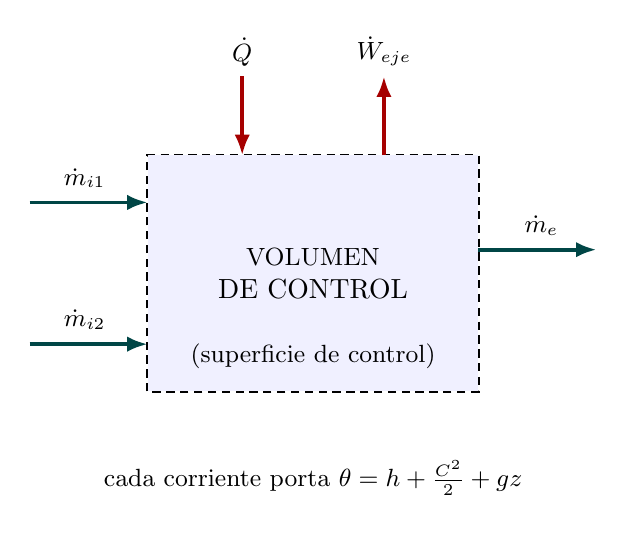
\begin{tikzpicture}[line width=1pt,>={Latex[length=2.6mm]}]
  \draw[densely dashed,line width=1.2pt] (0,0) rectangle (4.2,3.0);
  \fill[blue!6] (0,0) rectangle (4.2,3.0);
  \node[align=center] at (2.1,1.5){\small VOLUMEN\\DE CONTROL};
  \node at (2.1,0.45){\small (superficie de control)};
  % entradas
  \draw[->,teal!55!black,line width=1.4pt] (-1.5,2.4)--(0,2.4); \node[above] at (-0.8,2.45){\small $\dot m_{i1}$};
  \draw[->,teal!55!black,line width=1.4pt] (-1.5,0.6)--(0,0.6); \node[above] at (-0.8,0.65){\small $\dot m_{i2}$};
  % salidas
  \draw[->,teal!55!black,line width=1.4pt] (4.2,1.8)--(5.7,1.8); \node[above] at (5.0,1.85){\small $\dot m_{e}$};
  % calor y trabajo
  \draw[->,red!65!black,line width=1.3pt] (1.2,4.0)--(1.2,3.0); \node[above] at (1.2,4.0){\small $\dot Q$};
  \draw[->,red!65!black,line width=1.3pt] (3.0,3.0)--(3.0,4.0); \node[above] at (3.0,4.0){\small $\dot W_{eje}$};
  \node[align=center] at (2.1,-1.1){\small cada corriente porta $\theta=h+\tfrac{C^2}{2}+gz$};
\end{tikzpicture}
\end{document}
